
%(BEGIN_QUESTION)
% Copyright 2006, Tony R. Kuphaldt, released under the Creative Commons Attribution License (v 1.0)
% This means you may do almost anything with this work of mine, so long as you give me proper credit

Suppose you were connecting a HART-compliant transmitter to an indicator that was intolerant of the high-frequency HART communication signals.  Show where you would place a HART {\it filter} circuit in this 4-20 mA loop circuit to prevent those high-frequency signals from getting to the indicator, and also what that filter circuit would consist of:

$$\includegraphics[width=15.5cm]{i01398x01.eps}$$

\underbar{file i01398}
%(END_QUESTION)





%(BEGIN_ANSWER)

However you plan to filter the HART signals, resist the temptation to do this:

$$\includegraphics[width=15.5cm]{i01398x04.eps}$$

While placing a capacitor across the terminals of the indicator will bypass high-frequency AC HART signals around the indicator, it will also completely short out the HART data so the transmitter and communicator can't talk with one another!

I'll let you figure out a better method of HART signal filtering -- one that blocks HART frequencies from getting to the indicator without killing the HART signals throughout the network.

%(END_ANSWER)





%(BEGIN_NOTES)

There are two basic options: {\it block} or {\it bypass}.  First, the ``block'' option:

$$\includegraphics[width=15.5cm]{i01398x03.eps}$$

\vskip 10pt

\filbreak

Next, the ``bypass'' option:

$$\includegraphics[width=15.5cm]{i01398x02.eps}$$

%INDEX% Fieldbus, HART: filter circuit

%(END_NOTES)


